\documentclass[
  bibliography=totoc,     % Literatur im Inhaltsverzeichnis
  captions=tableheading,  % Tabellenüberschriften
  titlepage=firstiscover, % Titelseite ist Deckblatt
]{scrartcl}

\usepackage{fixltx2e}
\usepackage[aux]{rerunfilecheck}

\usepackage{polyglossia}
\setmainlanguage{german}

\usepackage{amsmath}
\usepackage{amssymb}
\usepackage{mathtools}

\usepackage{fontspec}
\defaultfontfeatures{Ligatures=TeX}

\usepackage[
  math-style=ISO,
  bold-style=ISO,
  sans-style=italic,
  nabla=upright,
  partial=upright,
]{unicode-math}

\usepackage[autostyle]{csquotes}

\usepackage[
  locale=DE,                   % deutsche Einstellungen
  separate-uncertainty=true,   % Immer Fehler mit \pm
  per-mode=symbol-or-fraction, % m/s im Text, sonst Brüche
]{siunitx}

\usepackage[version=3]{mhchem}

\usepackage{xfrac}

\usepackage[section, below]{placeins}
\usepackage[
  labelfont=bf,        % Tabelle x: Abbildung y: ist jetzt fett
  font=small,          % Schrift etwas kleiner als Dokument
  width=0.9\textwidth, % maximale Breite einer Caption schmaler
]{caption}
\usepackage{subcaption}
\usepackage{graphicx}
\usepackage{grffile}

\usepackage{float}
\floatplacement{figure}{htbp}
\floatplacement{table}{htbp}

\usepackage{booktabs}

\usepackage[
  unicode,
  pdfusetitle,    % Titel, Autoren und Datum als PDF-Attribute
  pdfcreator={},  % PDF-Attribute säubern
  pdfproducer={}, % "
]{hyperref}
\usepackage{bookmark}
\usepackage[shortcuts]{extdash}


\title{Bau einer einfachen Nebelkammer}
\subtitle{Ein Projekt der PeP et Al. Sommerakademie 2014}
\date{24. -- 31. August 2014}

\author{
  Vukan
  \texorpdfstring{\and}{,} Julian Wishahi
  \texorpdfstring{\and}{,} Johannes Kellers
}

\begin{document}
\maketitle
\section{Material}
Zum Aufbau der Nebelkammer wurden folgende Materialien verwendet:
\begin{itemize}
  \item 5 Glasplatten
  \item Silikon
  \item Styroporblock,  $\SI{1}{\meter}\cdot\SI{2}{\meter}\cdot\SI{0.2}{\meter}$
  \item Trockeneis, ca. \SI{6}{\kilo\gram}
  \item Metalplatte, ca. $\SI{25}{\centi\meter}\cdot\SI{25}{\centi\meter}$
  \item Panzertape 
  \item Filz + Neodym-Magnete zur Befestigung
  \item Knetmasse
  \item Isopropanol
\end{itemize}
\section{Aufbau}
Zu Beginn wurde aus den Glasplatten mithilfe von Silikon ein Aquarium gebaut.
Danach wurde der Styroporblock halbiert und übereinander befestigt. In den
oberen Block wurde eine Öffnung in der Größe der Metallplatte hereingeschnitten.
Die Metallplatte wurde mit schwarzem Klebenband beklebt, um einen möglichst
großen Kontrast zu ermöglichen. Als letzer Schritt des Aufbaus wurde das Filz
passend zugeschnitten und mithilfe von Magneten an der Unterseite des Aquariums
befestigt.

\section{Durchführung}
Um unsere Nebelkammer funktionsbereit zu machen, wurde der Filz in Isopropanol
getränkt. Des Weiteren wurde der Hohlraum im Styroporblock mit Trockeneis
gefüllt und die Metallplatte eingesetzt. Auf die Platte wurde das Aquarium
mithilfe von Knete luftdicht angebracht. Durch das Isopropanol an der Oberseite
entstand ein feiner Nebel, in dem Spuren von Teilchen beobachtet werden können.
Um die Nebelerzeugungsprozeß zu beschleunigen, kann die Oberseite mithilfe eines
Föhns erwärmt werden.

\section{Ergebnisse}
Es konnten zahlreiche Teilchenspuren beobachtet werden. Eine Zusammenstellung ist in Abbildung \ref{fig:nebelkammer} zu sehen.
\begin{figure}
  \centering
  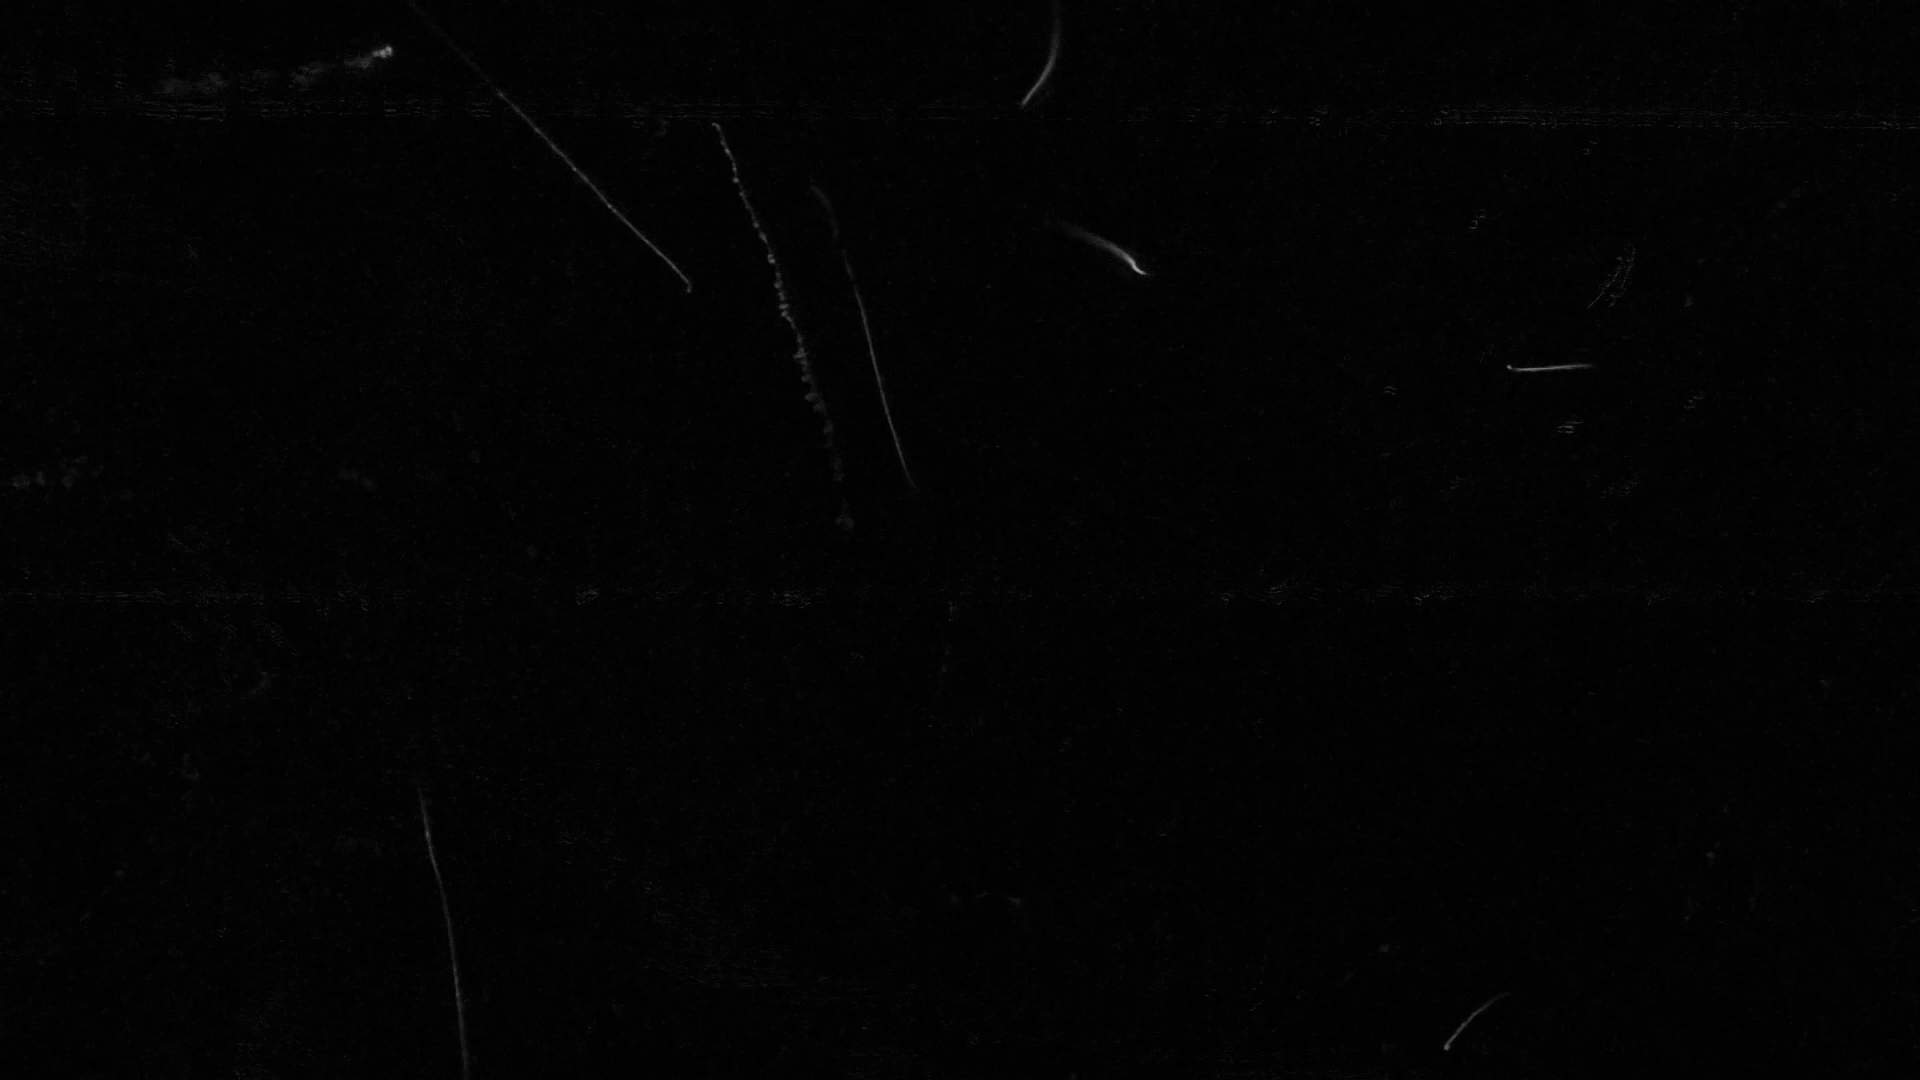
\includegraphics[width=\linewidth]{images/nebelkammer.png}
  \caption{Überblendendung von mehreren in der Nebelkammer beobachteten Spuren, aus Standbildern eines Videos extrahiert. Um die Spuren zu isolieren wurden von den Helligkeitswerten des Videos die Helligkeitswerte des um zwei Sekunden versetzten Videos subtrahiert.}
  \label{fig:nebelkammer}
\end{figure}


\section{Probleme und Verbesserungen}
Probleme, welche die Funktion der Nebelkammer stark unterbinden, traten nicht
auf. Jedoch gibt es zahlreiche Verbesserungsmöglichkeiten. Das Schneiden von
Styropor mithilfe von Cuttermessern und Sägen ist nicht optimal. Besser und
vorallen sauberer kann Styropor mit einem heißem Draht geschnitten werden. Das
Verkleben der Glaspaltten mit Silikon ist eine große Sauerei und kann durch den
Kauf eines bereits fertigen Aquariums umgangen werden. Für einen optimalen
Kontrast könnte die Metallplatte schwarz lackiert oder direkt eine schwarze
Platte verwendet werden. Das schwarze Klebeband erfüllt diesen Zweck nur
befriedigend. Verbesserungen können ebenfalls bei der Abdichtung zwischen der
Metallplatte und dem Aquarium erfolgen. Die verwendete Knete erfüllt diesen Job
nicht zufrieden stellend. Es kam durch diese Undichtigkeiten zu einem Luftzug
innerhalb der Nebelkammer, wodurch die Teilchen-Spuren nicht optimal detektiert
werden konnten. Als Alternative zur Knete könnten passende Gummidichtungen
verwendet werden. Des Weiteren könnte die Verbindung auch mit Silikon erfolgen.
Nachteil wäre dann, dass das Aquarium dauerhaft verbunden wäre. Zur Verbesserung
könnte das Aquarium auch mit einem dicht schließenem Deckel ausgestattet werden.
Als Trockeneis-Alternative könnte ein Peltier-Element benutzt werden.

\end{document}
